%% fcup-thesis.tex -- document template for PhD theses at FCUP
%%
%% Copyright (c) 2015 João Faria <joao.faria@astro.up.pt>
%%
%% This work may be distributed and/or modified under the conditions of
%% the LaTeX Project Public License, either version 1.3c of this license
%% or (at your option) any later version.
%% The latest version of this license is in
%%     http://www.latex-project.org/lppl.txt
%% and version 1.3c or later is part of all distributions of LaTeX
%% version 2005/12/01 or later.
%%
%% This work has the LPPL maintenance status "maintained".
%%
%% The Current Maintainer of this work is
%% João Faria <joao.faria@astro.up.pt>.
%%
%% This work consists of the files listed in the accompanying README.

%% SUMMARY OF FEATURES:
%%
%% All environments, commands, and options provided by the `ut-thesis'
%% class will be described below, at the point where they should appear
%% in the document.  See the file `ut-thesis.cls' for more details.
%%
%% To explicitly set the pagestyle of any blank page inserted with
%% \cleardoublepage, use one of \clearemptydoublepage,
%% \clearplaindoublepage, \clearthesisdoublepage, or
%% \clearstandarddoublepage (to use the style currently in effect).
%%
%% For single-spaced quotes or quotations, use the `longquote' and
%% `longquotation' environments.


%%%%%%%%%%%%         PREAMBLE         %%%%%%%%%%%%

%%  - Default settings format a final copy (single-sided, normal
%%    margins, one-and-a-half-spaced with single-spaced notes).
%%  - For a rough copy (double-sided, normal margins, double-spaced,
%%    with the word "DRAFT" printed at each corner of every page), use
%%    the `draft' option.
%%  - The default global line spacing can be changed with one of the
%%    options `singlespaced', `onehalfspaced', or `doublespaced'.
%%  - Footnotes and marginal notes are all single-spaced by default, but
%%    can be made to have the same spacing as the rest of the document
%%    by using the option `standardspacednotes'.
%%  - The size of the margins can be changed with one of the options:
%%     . `narrowmargins' (1 1/4" left, 3/4" others),
%%     . `normalmargins' (1 1/4" left, 1" others),
%%     . `widemargins' (1 1/4" all),
%%     . `extrawidemargins' (1 1/2" all).
%%  - The pagestyle of "cleared" pages (empty pages inserted in
%%    two-sided documents to put the next page on the right-hand side)
%%    can be set with one of the options `cleardoublepagestyleempty',
%%    `cleardoublepagestyleplain', or `cleardoublepagestylestandard'.
%%  - Any other standard option for the `report' document arclass can be
%%    used to override the default or draft settings (such as `10pt',
%%    `11pt', `12pt'), and standard LaTeX packages can be used to
%%    further customize the layout and/or formatting of the document.

%% *** Add any desired options. ***
%PDF
%\documentclass[a4paper,narrowmargins,12pt,oneside,draft,onehalfspaced,singlespacednotes]{fcup-thesis}
%\documentclass[a4paper,narrowmargins,12pt,oneside,onehalfspaced,singlespacednotes]{fcup-thesis}
%Print
%\documentclass[draft,a4paper,narrowmargins,12pt,twoside,openright,onehalfspaced,singlespacednotes]{fcup-thesis}
\documentclass[a4paper,narrowmargins,12pt,twoside,openright,onehalfspaced,singlespacednotes]{fcup-thesis}

%% *** Add \usepackage declarations here. ***
%% The standard packages `geometry' and `setspace' are already loaded by
%% `ut-thesis' -- see their documentation for details of the features
%% they provide.  In particular, you may use the \geometry command here
%% to adjust the margins if none of the ut-thesis options are suitable
%% (see the `geometry' package for details).  You may also use the
%% \setstretch command to set the line spacing to a value other than
%% single, one-and-a-half, or double spaced (see the `setspace' package
%% for details).
% Overfull statements
\pretolerance=150
\setlength{\emergencystretch}{3em}
% Overfull end
\usepackage[english]{babel}
\usepackage{lipsum}
\usepackage[utf8]{inputenc}


%%% Additional useful packages
%%% ----------------------------------------------------------------
\usepackage{array}
\usepackage{amsmath}  
\usepackage{amssymb}
\usepackage{amsfonts}
\DeclareFontFamily{OT1}{pzc}{}
\DeclareFontShape{OT1}{pzc}{m}{it}{<-> s * [0.900] pzcmi7t}{}
\DeclareMathAlphabet{\mathpzc}{OT1}{pzc}{m}{it}
\usepackage{amsthm}      
\usepackage[ruled,algochapter]{algorithm2e}
\usepackage{algorithmic}
\usepackage{bm}
\usepackage[mathscr]{euscript}
\usepackage{graphicx}       
\usepackage{psfrag}         
\usepackage{fancyvrb}    
\usepackage{float}
\usepackage{ltablex}
\usepackage[square,sort,comma,numbers]{natbib}        
\usepackage{bbding}         
\usepackage{dcolumn}        
\usepackage{booktabs} 
\usepackage{multirow}
\usepackage{paralist}     
\usepackage{ifdraft}  
\usepackage{indentfirst}    
\usepackage[nottoc,notlof,notlot]{tocbibind}
\usepackage{url}
\usepackage{tabularx}
\usepackage{subcaption}
\usepackage[unicode]{hyperref}
\usepackage{xcolor}

\hypersetup{pdftitle=LiDAR obstacle detection and avoidance, 
            pdfauthor=Alojz Gomola,
            colorlinks=false,
            urlcolor=blue,
            pdfstartview=FitH,
            pdfpagemode=UseOutlines,
            pdfnewwindow,
            breaklinks
          }
\usepackage{array}
\newcolumntype{L}[1]{>{\raggedright\let\newline\\\arraybackslash\hspace{0pt}}m{#1}}
\newcolumntype{C}[1]{>{\centering\let\newline\\\arraybackslash\hspace{0pt}}m{#1}}
\newcolumntype{R}[1]{>{\raggedleft\let\newline\\\arraybackslash\hspace{0pt}}m{#1}}         
\newcolumntype{B}{X}
\newcolumntype{S}[1]{>{\hsize=#1\textwidth}X}

\newcommand{\FIGDIR}{./Pics}    %%% directory containing figures
\newcommand{\twolinecellr}[2][r]{%
  \begin{tabular}[#1]{@{}r@{}}#2\end{tabular}}
\newcommand{\secState}[1]{
	\ifdraft{(#1) }{}
}
\theoremstyle{plain}
\newtheorem{theorem}{Theorem}
\newtheorem{lemma}[theorem]{Lemma}
\newtheorem{proposition}[theorem]{Proposition}

\theoremstyle{plain}
\newtheorem{definition}{Definition}
\newtheorem{problem}{Problem}
\newtheorem{example}{Example}
\newtheorem{assumption}{Assumption}

\theoremstyle{remark}
\newtheorem*{corollary}{Corollary}
\newtheorem*{note}{Note}




\newenvironment{dokaz}{
  \par\medskip\noindent
  \textit{Proof}.
}{
\newline
\rightline{\SquareCastShadowBottomRight}
}

\newenvironment{constraints}[1]{
  \par\medskip\noindent
  \textit{Constraints #1} \\
}{
\newline
\rightline{\SquareCastShadowBottomRight}
}


%\bibliographystyle{plainnat}     %% Author (year) style
\bibliographystyle{unsrt}        %% [number] style
\setcitestyle{square}

% Section  3.7 Challenge list
\newif\ifproblemchallenge   %# Build block for problem challenges
\problemchallengetrue       %# Show comments

\newcommand{\R}{\mathbb{R}}
\newcommand{\N}{\mathbb{N}}

\DeclareMathOperator{\pr}{\textsf{P}}
\DeclareMathOperator{\E}{\textsf{E}\,}
\DeclareMathOperator{\var}{\textrm{var}}
\DeclareMathOperator{\sd}{\textrm{sd}}


\newcommand{\T}[1]{#1^\top}        

\newcommand{\goto}{\rightarrow}
\newcommand{\gotop}{\stackrel{P}{\longrightarrow}}
\newcommand{\maon}[1]{o(n^{#1})}
\newcommand{\abs}[1]{\left|{#1}\right|}
\newcommand{\dint}{\int_0^\tau\!\!\int_0^\tau}
\newcommand{\isqr}[1]{\frac{1}{\sqrt{#1}}}
\newcommand{\norm}[1]{\left\lVert#1\right\rVert}


\newcommand{\pulrad}[1]{\raisebox{1.5ex}[0pt]{#1}}
\newcommand{\mc}[1]{\multicolumn{1}{c}{#1}}
\newcommand{\TBD}[1]{\color{red}\emph{--TBD:}#1\color{black}}

%%%%%%%%%%%%%%%%%%%%%%%%%%%%%%%%%%%%%%%%%%%%%%%%%%%%%%%%%%%%%%%%%%%%%%%%
%%                                                                    %%
%%                   ***   I M P O R T A N T   ***                    %%
%%                                                                    %%
%%  Fill in the following fields with the required information:       %%
%%   - \degree{...}       name of the degree obtained                 %%
%%   - \department{...}   name of the graduate department             %%
%%   - \gradyear{...}     year of graduation                          %%
%%   - \author{...}       name of the author                          %%
%%   - \title{...}        title of the thesis                         %%
%%%%%%%%%%%%%%%%%%%%%%%%%%%%%%%%%%%%%%%%%%%%%%%%%%%%%%%%%%%%%%%%%%%%%%%%

%% *** Change this example to appropriate values. ***
\degree{Doctor of Philosophy}
\department{Departamento de Matem\'{a}tica}
\gradyear{2019}
\author{Alojz Gomola}
\title{Obstacle Avoidance Framework based on Reach Sets}

%% *** NOTE ***
%% Put here all other formatting commands that belong in the preamble.
%% In particular, you should put all of your \newcommand's,
%% \newenvironment's, \newtheorem's, etc. (in other words, all the
%% global definitions that you will need throughout your thesis) in a
%% separate file and use "\input{filename}" to input it here.


%% *** Adjust the following settings as desired. ***

%% List only down to subsections in the table of contents;
%% 0=chapter, 1=section, 2=subsection, 3=subsubsection, etc.
\setcounter{tocdepth}{3}

%% Make each page fill up the entire page.
\flushbottom


%%%%%%%%%%%%      MAIN  DOCUMENT      %%%%%%%%%%%%

\begin{document}


%%%%%%%%%%%%%%%%%%%%%%%%%%%%%%%%%%%%%%%%%%%%%%%%%%%%%%%%%%%%%%%%%%%%%%%%
%%  Put your Chapters here; the easiest way to do this is to keep     %%
%%  each chapter in a separate file and `\include' all the files.     %%
%%  Each chapter file should start with "\chapter{ChapterName}".      %%
%%  Note that using `\include' instead of `\input' will make each     %%
%%  chapter start on a new page, and allow you to format only parts   %%
%%  of your thesis at a time by using `\includeonly'.                 %%
%%%%%%%%%%%%%%%%%%%%%%%%%%%%%%%%%%%%%%%%%%%%%%%%%%%%%%%%%%%%%%%%%%%%%%%%

%% *** Include chapter files here. ***

\setcounter{chapter}{6}
\setcounter{section}{1}
%06-Approach

    %06-03 Movement Automaton
    \cleardoublepage
\section{\secState{R}UAS Model and Control}\label{s:modelMAImplementation}

\noindent The key feature of \emph{Movement Automaton} is to interface \emph{continuous-control signal} as the \emph{discrete command chain}. Following topics are introduced in this section:

\begin{enumerate}
    \item \emph{UAS Nonlinear Model} (sec. \ref{s:UASNonlinearModel}) - simple plane model used in this work as \emph{controlled plant}.
    
    \item \emph{Movement Automaton} (sec. \ref{s:movementAutomatonDefinition}) - movement automaton for \emph{UAS Nonlinear Model} constructed from scratch.
    
    \item \emph{Segmented Movement Automaton} (sec. \ref{s:segmentedMovementAutomaton}) - for more complex systems the \emph{State Space} can be \emph{separated into Segments} and \emph{segment movement automaton} is used to generate \emph{thick reference trajectory}.
    
    \item \emph{Reference Trajectory Generator} (sec. \ref{s:referenceTrajectoryGenerator}) - other use of \emph{Movement Automaton} as predictor for \emph{reference trajectory calculation}.
\end{enumerate}


\subsection{\secState{R}UAS Nonlinear Model}\label{s:UASNonlinearModel}
\paragraph{Motivation:} Simplified rigid body kinematic model will be used. This model have decoupled roll, yaw and pitch angles. The focus is on \emph{reach set approximation methods}, therefore \emph{UAS model} is simplified.

\paragraph{State Vector} (eq. \ref{eq:simple3dStatevector}) defined as positional state in euclidean position in right-hand euclidean space, where \emph{x, y, z} can be abstracted as latitude, longitude, altitude.
\begin{equation}\label{eq:simple3dStatevector}
    state = \left [ x,y,z, roll, pitch, yaw \right]^T
\end{equation}


\paragraph{Input Vector} (eq. \ref{eq:simple3dInputVector}) is defined as linear velocity of UAS $v$ and angular speed of rigid body $\omega_{roll}, \omega_{pitch},\omega_{yaw}$.

\begin{equation}\label{eq:simple3dInputVector}
    input = \left [ v, \omega_{roll}, \omega_{pitch},\omega_{yaw}\right ]^T
\end{equation}


\noindent Velocity distribution function (eq. \ref{eq:simple3dvelocityDistribution})  is is defined trough standard rotation matrix  and linear velocity $v$, oriented velocity [$v_x$, $v_y$, $v_z$] given by (eq. \ref{eq:UASNonlinearModelSimple}).

\begin{equation}\label{eq:simple3dvelocityDistribution}
    \begin{bmatrix}
    v_x\\
    v_y\\
    v_z\
    \end{bmatrix}
    =
    \begin{bmatrix}
         v\cos(pitch)\cos(yaw)\\
         v\cos(pitch)\sin(yaw)\\
         -v\sin(pitch)\\
    \end{bmatrix}
\end{equation}

\paragraph{UAS Nonlinear Model} (eq. \ref{eq:UASNonlinearModelSimple}) is given by \emph{first order equations:}

\begin{equation}\label{eq:UASNonlinearModelSimple}
    \begin{aligned}
        \frac{\partial x}{\partial time} &= v\cos(pitch)\cos(yaw);\\
        \frac{\partial y}{\partial time} &= v\cos(pitch)\sin(yaw);\\
        \frac{\partial z}{\partial time} &= -v\sin(pitch);\\
    \end{aligned}\\\quad\quad
    \begin{aligned}
        \frac{\partial roll}{\partial time} &= \omega_{roll};\\
        \frac{\partial pitch}{\partial time} &= \omega_{pitch};\\
        \frac{\partial yaw}{\partial time} &= \omega_{yaw};\\
    \end{aligned}
\end{equation}

\subsection{\secState{R}Movement Automaton for UAS Model}\label{s:movementAutomatonDefinition}

\paragraph{Motivation:} An \emph{UAS Nonlinear Model} (eq. \ref{eq:UASNonlinearModelSimple}) can be modeled by \emph{Movement Automaton} (def. \ref{def:movementAutomaton}). 

\paragraph{Movement Primitives} by (def. \ref{def:MovementPrimitive})  are given as (eq. \ref{eq:movementPrimitive}). To define primitives the \emph{minimal time} is $1 s$. The \emph{maximal duration} is also $1s$. 

\begin{assumption}\label{ass:transitionTime}
    Let assume that \emph{transition time} of \emph{roll, pitch, yaw, linear velocity} is $0 s$.
\end{assumption}

Under the assumption (as. \ref{ass:transitionTime}) the \emph{movement transitions} (def. \ref{def:movementTransition}) have $0$ duration.

\begin{note}
    The assumption (as. \ref{ass:transitionTime}) can be relaxed under condition that \emph{path tracking controller exists}.
\end{note}

\paragraph{Movements} (def. \ref{def:Movement}) for \emph{fixed step} $k$ we start with discretization of the input variables.

\noindent The \emph{linear velocity} in text step is given:
\begin{equation}\label{eq:applyMovement}
    v(k+1) = v(k) +\delta v(k)
\end{equation}

\noindent The \emph{roll, pitch, yaw} for next step are given 

\begin{equation}\label{eq:applyMovement1}
    \begin{aligned}
        roll(k+1)  &= roll(k) + \delta roll(k)\\
        pitch(k+1) & = pitch(k) + \delta pitch(k)\\
        yaw(k+1) & = yaw(k) + \delta yaw(k)\\
    \end{aligned}    
\end{equation}

\noindent The $\delta v(k)$ is \emph{velocity change}, $\delta roll(k)$, $\delta pitch(k)$, $\delta yaw(k)$, are \emph{orientation changes} for current discrete step $k$. If the duration of \emph{transition} is $0 s$ (as. \ref{ass:transitionTime}) then 3D trajectory evolution in discrete time is given as: 

\begin{equation}\label{eq:applyMovement2}
    \begin{aligned}
        x(k+1)&= x(k) + v(k+1) \cos(pitch(k+1)) \cos(yaw(k+1)) & = \delta x(k)\\
        y(k+1)&= y(k) + v(k+1) \cos(pitch(k+1)) \sin(yaw(k+1)) & = \delta y(k)\\
        z(k+1)&= z(k) - v(k+1) \sin(pitch(k+1))                & = \delta z(k)\\
        time(k+1)& = time(k)+1                                & = \delta time(k)
    \end{aligned}    
\end{equation}

\noindent The $\delta x(k)$, $\delta y(k)$, $\delta z(k)$ are positional differences depending on \emph{input vector} for given discrete time $k$:
\begin{equation}\label{eq:ourImput}
    input(k) = \left[
                    \begin{gathered}
                    \delta x(k), \delta y(k), \delta z(k), \delta v (k),\\
                    \delta roll (k), \delta pitch(k), \delta yaw(k),\delta time (k)
                    \end{gathered} 
                \right]^T
\end{equation}

\noindent The \emph{state vector} for discrete time is given:
\begin{equation}\label{eq:ourState}
    state(k) = \left[
                    \begin{gathered}
                     x(k),  y(k),  z(k),  v (k),\\
                     roll (k),  pitch(k),  yaw(k), time (k)
                    \end{gathered} 
                \right]^T
\end{equation}

\noindent The nonlinear model (eq. \ref{eq:UASNonlinearModelSimple}) is then reduced to \emph{linear discrete model} (eq. \ref{eq:uasLinearDiscreteModel}) given by \emph{apply movements} function (eq. \ref{eq:applyMovement}, \ref{eq:applyMovement1}, \ref{eq:applyMovement2}).

\begin{equation}\label{eq:uasLinearDiscreteModel}
    state(k+1) = applyMovement(state(k), input(k)) 
\end{equation}

\paragraph{Movement Set} for linear discrete model (eq. \ref{eq:uasLinearDiscreteModel}) is defined as set of extreme unitary movements on main axes (tab. \ref{tab:movements1}) and diagonal axes (tab. \ref{tab:movements2}).

\begin{table}[H]
    \centering
    \begin{tabular}{r||r|r|r|r|r}
    
        $input(movement)$           &    Straight  & Down & Up & Left  & Right   \\\hline\hline
        $\delta     x(k)[m]$           &    1.00	  & 0.98  & 0.98  & 0.98 & 0.98  \\\hline
        $\delta     y(k)[m]$           &    0	      & 0	  & 0	  & 0.13 & -0.13 \\\hline
        $\delta     z(k)[m]$           &    0	      & -0.13 & 0.13  &	0	 & 0     \\\hline
        $\delta  roll(k) [^\circ]$	   &    0	      & 0	  & 0	  & 0    & 0     \\\hline
        $\delta pitch(k) [^\circ]$     &    0	      & $15^\circ$  & -$15^\circ$ & 0	 & 0     \\\hline
        $\delta   yaw(k) [^\circ]$     &    0	      & 0	  & 0	  & $15^\circ$ & -$15^\circ$ \\
    \end{tabular}
    \caption{Input values for main axes movements.}
    \label{tab:movements1}
\end{table}
\begin{table}[H]
    \centering
    \begin{tabular}{r||r|r|r|r}
        $input(movement)$             & Down-Left & Down-Right & Up-Left  & Up-Right   \\\hline\hline
        $\delta     x(k)[m]$           & 0.76  & 0.76  & 0.76 & 0.76  \\\hline
        $\delta     y(k)[m]$           & -0.13	& 0.13	& 0.13 & -0.13 \\\hline
        $\delta     z(k)[m]$           & -0.13 & -0.13 & 0.13 & 0.13  \\\hline
        $\delta  roll(k) [^\circ]$	& 0	    & 0	    & 0    & 0     \\\hline
        $\delta pitch(k) [^\circ]$     & -$15^\circ$ & -$15^\circ$ & $15^\circ$ & $15^\circ$     \\\hline
        $\delta   yaw(k) [^\circ]$    & $15^\circ$	& -$15^\circ$	& $15^\circ$ & -$15^\circ$ \\
    \end{tabular}
    \caption{Input values for diagonal axes movements.}
    \label{tab:movements2}
\end{table}

\begin{note}
    \emph{Movement set} in shorten form is given as
    \begin{equation}\label{eq:OurMovementSet}
        Movement Set= \left\{
        \begin{gathered}
            Straight, Left,Right, Up, Down,\\
            Down Left, Down Right,  Up Left,   Up Right
        \end{gathered}
        \right\}
    \end{equation}
\end{note}

\paragraph{Trajectory} by (def. \ref{def:MovementAutomatonTrajectory}) for initial time $time = 0$ , initial state $state(0)$ and \emph{Movement Buffer} (from def. \ref{def:MovementBuffer}):
\begin{equation}\label{eq:ourBuffer}
    Buffer \in Movement Set^* (eq. \ref{eq:OurMovementSet}), \quad  |Buffer| \in \N
\end{equation}

\noindent Trajectory (eq. \ref{eq:ourTrajectoryImplementation}) is then given as the time-series of discrete states:
\begin{equation}\label{eq:ourTrajectoryImplementation}
    Trajectory(state(0),Buffer)= \left\{\begin{gathered}state(0)+\sum_{j=0}^{i-1} input(movement(j)):\\i \in\left\{1\dots |Buffer|+1\right\}, \\movement(\cdot) \in Buffer\end{gathered}\right\}
\end{equation}

\noindent Trajectory (eq. \ref{eq:ourTrajectoryImplementation}) is ordered set of states bounded to discrete time $0\dots n$ , where $n$ is member count of \emph{Buffer}. Trajectory set has $n+1$ members:

\begin{equation}
    \begin{aligned}
    T&rajectory(state(0),Buffer)=\\
        &\left\{
        \begin{aligned}
            state(0) &= state(0) + \{\}\\
            state(1) &= state(0) + input(movement(1))\\
            state(2) &= state(0) + input(movement(1)) +input(movement(2))\\
             \vdots  &= \vdots\\
            state(n) &= state(0) + input(movement(1))+\dots+input(movement(n))\\
        \end{aligned}
        \right\}
    \end{aligned}
\end{equation}

\paragraph{State Projection} (eq. \ref{eq:ourStateProjection}) for the \emph{Trajectory} (eq. \ref{eq:ourTrajectoryImplementation}) is given as follow:
\begin{equation}\label{eq:ourStateProjection}
    StateProjection(Trajectory,time) = Trajectory.getMemberByIndex(time+1)
\end{equation}

\begin{note}
    \emph{Movement Automaton} for system (eq. \ref{eq:UASNonlinearModelSimple}) with given (as. \ref{ass:transitionTime}) is established with all related properties (sec. \ref{def:movementAutomaton}).
\end{note}

\newpage
\subsection{\secState{R}Segmented Movement Automaton}\label{s:segmentedMovementAutomaton}
\paragraph{Motivation:} Constructing \emph{Movement Automaton} for more complex system can be tedious. Used \emph{Movement Automaton} for \emph{UAS system} (\ref{eq:UASNonlinearModelSimple}) has decoupled control which is not true for most of the copters/planes \cite{fossen2011mathematical}.

\paragraph{Partitioning UAS State Space:} Proposed movement automaton is defined by its Movement set (tab. \ref{tab:movements1},\ref{tab:movements2}). Those can be scaled depending on maneuverability in the  \emph{Initial state} $state(0)$:
\begin{enumerate}
    \item \emph{Climb/Descent Rate} $\delta pitch_{max}(k)$ - the maximal climb or descent rate for Up/Down movements.
    \item \emph{Turn Rate} $\delta yaw_{max}(k)$ - the maximal turn rate for Left/Right movement.
    \item \emph{Acceleration} $\delta v_{max}(k)$ - the maximal acceleration in cruising speed range.
\end{enumerate}

\begin{definition}{State Space partition}\label{def:stateSpacePartition}
    \emph{Maneuverability} is depending on \emph{Initial State}. There can not be the infinite count of \emph{Movement Automatons}.
    
    The state space $State Space \in \R^n$ can be separated into two exclusive subsets:
    \begin{equation}
        StateSpace = [ImpactStates, NonImpactingStates]
    \end{equation}
    
    The \emph{Impacting states} are states which bounds the \emph{Maneuverability}: $\delta pitch_{max}(k)$, $\delta yaw_{max}(k)$, $\delta v_{max}(k)$. For each \emph{impact state} is possible to define upper and lower boundary:
    \begin{multline}
        \forall impactState\in ImpactStates, \exists:\\ lower(impactState) \le value(impactState) \le upper(impactState) 
    \end{multline}
    
	\noindent    The bounded interval of impact state can be separated into distinctive \emph{impact state segments} like follow:
    \begin{multline}
        impactState\in [lower,upper]:\\ \{[lower,separator_1[\dots\cup\dots[separator_i,separator_{i+1}[\dots\cup\dots\\\dots\cup\dots[separator_n,upper]\}=\\
        = impactStateIntervals(impactState)
    \end{multline}
    \begin{note}
        The interval length depends on model dynamics. The rule of thumb is to keep maximal climb/descend/turn/acceleration rates near constant value. 
    \end{note}
        
\noindent When partitioning of \emph{all impact States} finishes, the count of partitions is given as product of \emph{count of partitions} for each member of \emph{Impact States}:
    
    \begin{equation}
        partition Count = \prod_{impactState \in}^{ImpactStates} |impactStateIntervals(impactState)| 
    \end{equation}
    
    \begin{note}
        Try to keep the count of partitions to minimum, each new interval increases the count of partitions geometrically. 
    \end{note}
    
    There is finite number $n$ of \emph{Impacting States}, these are separated into $impactState-$ $Intervals_i$ with respective index $i \in 1\dots n$. The \emph{segment} with index defining position used \emph{impacting state} intervals is given as \emph{constrained space}:
    
    \begin{equation}
        Segment(index) = \left[
            \begin{gathered}
                impactState_1 \in impactStateIntervals_1[index_1],\\
                \vdots\\
                impactState_n \in impactStateIntervals_n[index_n],\\
                \vdots\\
                NonImpactingStates    
                \end{gathered}\right]
    \end{equation}
    
    Each \emph{Segment} covers one of impacting state intervals combination, because the original intervals are exclusive, also \emph{Segments} are exclusive. The \emph{union} of all segments covers \emph{State Space}:
    
    \begin{equation}\label{eq:segmentedStateSpace}
        StateSpace = \bigcup_{\forall\quad index \in |impactStateIntervals|^n} Segment(index)
    \end{equation}
\end{definition}

\paragraph{Segmented Movement Automaton:} The segmentation of \emph{state space} is done  in (def. \ref{def:stateSpacePartition}) any \emph{state} belongs exactly to \emph{Segment} of \emph{State Space}. For each \emph{Segment} in \emph{State Space}it is possible to assess: \emph{Climb/Descent Rate} $\delta pitch_{max}(k)$, \emph{Turn Rate} $\delta yaw_{max}(k)$, and, \emph{Acceleration} $\delta v_{max}(k)$.


\begin{definition}{Movement Automaton for Segment(index)}\label{def:segmentMovementAutomaton}
    

\noindent For for Model(eq. \ref{eq:uasLinearDiscreteModel}) with State (eq. \ref{eq:ourState}) the input vector (eq. \ref{eq:ourImput}) is for position $[x,y,z]$ and velocity defined like: 

\begin{equation}
    \begin{aligned}
        \delta x(k)& = \left(v(k)+\delta v(k)\right) \cos(\delta pitch(k)) \cos(\delta yaw(k))\\
        \delta y(k)& = \left(v(k)+\delta v(k)\right) \cos(\delta pitch(k)) \sin(\delta yaw(k))\\
        \delta z(k)& = -\left(v(k)+\delta v(k)\right)\cos(\delta pitch(k))\\
        \delta v(k)&\in [-\delta v(k)_{max},\delta v(k)_{max}]
    \end{aligned}
\end{equation}
\end{definition}

\noindent The acceleration $\delta v(k)$ is in interval $[-\delta v(k)_{max},\delta v(k)_{max}]$, usually set to 0 $ms^{-1}$. The change of the orientation angles for \emph{Movement Set} (eq. \ref{eq:OurMovementSet}) is given in (tab. \ref{tab:movements3},\ref{tab:movements4}).

\begin{table}[H]
    \centering
    \begin{tabular}{r||r|r|r|r|r}
    
        $input(movement)$           &    Straight  & Down & Up & Left  & Right   \\\hline\hline
        $\delta  roll(k) [^\circ]$	   &    0	      & 0	  & 0	  & 0    & 0     \\\hline
        $\delta pitch(k) [^\circ]$     &    0	      & $\delta pitch_{max}$  & -$\delta pitch_{max}$ & 0	 & 0     \\\hline
        $\delta   yaw(k) [^\circ]$     &    0	      & 0	  & 0	  & $\delta yaw_{max}$ & -$\delta yaw_{max}$ \\
    \end{tabular}
    \caption{Orientation input values for main axes movements.}
    \label{tab:movements3}
\end{table}


\begin{table}[H]
    \centering
    \begin{tabular}{r||r|r|r|r}
        $input(movement)$             & Down-Left & Down-Right & Up-Left  & Up-Right   \\\hline\hline

        $\delta  roll(k) [^\circ]$	& 0	    & 0	    & 0    & 0     \\\hline
        $\delta pitch(k) [^\circ]$     & -$\delta pitch_{max}$ & -$\delta pitch_{max}$ & $\delta pitch_{max}$ & $\delta pitch_{max}$     \\\hline
        $\delta   yaw(k) [^\circ]$    & $\delta yaw_{max}$	& -$\delta yaw_{max}$	& $\delta yaw_{max}$ & -$\delta yaw_{max}$ \\
    \end{tabular}
    \caption{Orientation input values for diagonal axes movements.}
    \label{tab:movements4}
\end{table}

\begin{note}
    The \emph{Trajectory} is calculated same as in (eq. \ref{eq:ourTrajectoryImplementation}). The \emph{State Projection} is given as in (eq. \ref{eq:ourStateProjection}).
\end{note}

\noindent Then the \emph{Movement Automaton} for \emph{Segment} $\in$ \emph{State Space} is defined.

\begin{definition}{Segmented Movement Automaton}\label{def:segmentedMovementAutomaton}
    For system with segmented state space (eq. \ref{eq:segmentedStateSpace}) there is for each $state(k)$ in $StateSpace$ injection function:
    \begin{equation} \label{eq:activeMovementAutomaton}
        ActiveMovementAutomaton:StateSpace\to MovementAutomaton
    \end{equation}
    
\noindent Selecting appropriate \emph{movement automaton} implementation (def. \ref{def:segmentMovementAutomaton}) for \emph{state(k)} $\in$ \emph{Segment} $\subset$ \emph{State Space}. The mapping function (eq. \ref{eq:activeMovementAutomaton}) is injection mapping every state(k) to Segment then \emph{Movement Automaton Implementation}. The trajectory generated is then given:
    
    \begin{equation}\label{eq:ourTrajectoryImplementationSegmented}
        Trajectory\left(\begin{gathered}state(0),\\Buffer\end{gathered}\right)= 
        \left\{
            \begin{gathered}
                state(0)+\dots\\\sum_{j=0}^{i-1} 
                    \begin{aligned} 
                        &ActiveMovementAutomaton(state(j-1)).\\
                        &\quad.input(movement(j))
                    \end{aligned}:\\
                i \in\left\{1\dots |Buffer|+1\right\}, \\
                movement(\cdot) \in Buffer
            \end{gathered}
        \right\}
    \end{equation}
    
\end{definition}

\newpage
\subsection{\secState{R}Reference Trajectory Generator}\label{s:referenceTrajectoryGenerator}

\paragraph{Reference Trajectory Generator:} Segmented Movement Automaton (def.  \ref{def:segmentedMovementAutomaton}) with \emph{trajectory function} (eq. \ref{eq:ourTrajectoryImplementationSegmented}) is used as \emph{reference trajectory generator} for \emph{complex systems}. 

There is assumption that precise \emph{path tracking} implementation exist for such system which with \emph{thick reference trajectory} gives similar results to \emph{plain movement automaton control}.

The \emph{Reference trajectory} (eq. \ref{eq:generatedReferenceTrajectory}) for \emph{Planned} movement set is given as projection  of \emph{Trajectory} time series to position time series $[x,y,z,t]$:

\begin{equation}\label{eq:generatedReferenceTrajectory}
    Reference Trajectory:Trajectory\left(\begin{gathered}state(now),\\Planned\end{gathered}\right) 
    \to 
    \begin{bmatrix}
        x_{ref} \in \R^{|Planned|}\\
        y_{ref} \in \R^{|Planned|}\\
        z_{ref} \in \R^{|Planned|}\\
        t_{ref} \in \R^{|Planned|}
    \end{bmatrix}
\end{equation}

\paragraph{Predictor:} The \emph{Reference Trajectory Generator} (eq. \ref{eq:generatedReferenceTrajectory}) can be also used as predictor. 

\begin{note}
    The \emph{Segmented Movement Automaton} (def. \ref{def:segmentedMovementAutomaton}) is used in this work with one Segment equal to State space with input function given by (\ref{tab:movements1}, \ref{tab:movements2}). The predictor used in \emph{Reach set computation} is given by (eq. \ref{eq:generatedReferenceTrajectory}).
\end{note}

    	\subsection{\secState{R}Movement Automaton Applications}\label{sec:MovementAutomatonBackground}

    \noindent\emph{Movement Automaton} is basic interface approach for discretization of \emph{trajectory evolution}  or \emph{control input} for any \emph{continuous or discrete system model}.
    
    \emph{Main function} of \emph{Movement Automaton is} for system given by equation $\dot{state}=f(time,state,input)$ with initial state $state_0$ to generate \emph{reference trajectory} $\hat{state}(t)$ or \emph{control signal} $input(t)$.
    
    Using \emph{Movement Automaton} as \emph{Control Proxy} will provide us with \emph{discrete command chain} interface. This will reduce the \emph{non deterministic} element from \emph{Evasive trajectory} generation, by reducing infinite maneuver set to finite \emph{movement set}.
    
    \emph{Non determinism} of \emph{Avoidance Maneuver} have been discussed as an issue in following works:
    \begin{enumerate}
        \item Newton gradient method for evasive car maneuvers \cite{vsantin2011combined}.
        \item Non-holistic methods for trajectory generation \cite{pin1990autonomous}.
        \item Stochastic approach to elliptic trajectories generation \cite{andrzejak2001epileptic}.
    \end{enumerate}
    
\noindent\emph{Examples} of \emph{Movement Automaton Implementation} as \emph{Control Element} can be mentioned as follows:
    \begin{enumerate}
        \item Control of traffic flow \cite{kuwata2009real}.
        \item Complex air traffic collision situation resolution system  \cite{frazzoli2001robust,frazzoli2000trajectory}.
        \item SAA/DAA capable avoidance system \cite{gomola2017obstacle}.
    \end{enumerate}



    	\section{Specialization of Hybrid Automaton}\label{s:MovementAutomatonBuidlingBlocks}

\paragraph{Idea:} There is  a need for \emph{fast trajectory approximation} method. The basic idea is taken from the pilot steering a plane. The pilot has issued commands from a navigator in a very short and precise manner. The movement has its primitive phase when steering is static, and its transition phase when steering is moving from one static position to another. 

Imagine having vertical and horizontal flaps an on airplane (fig. \ref{fig:movementsExample}). The \emph{navigator} is issuing a command every second to a pilot. Hands of the pilot translate each command to an input signal (blue line). The command validity period (black frame) is split into \emph{transition period} (red frame) when the input signal is changing and primitive period (magenta frame) when the position of the input signal is static.
 
\begin{figure}[H]
    \centering
    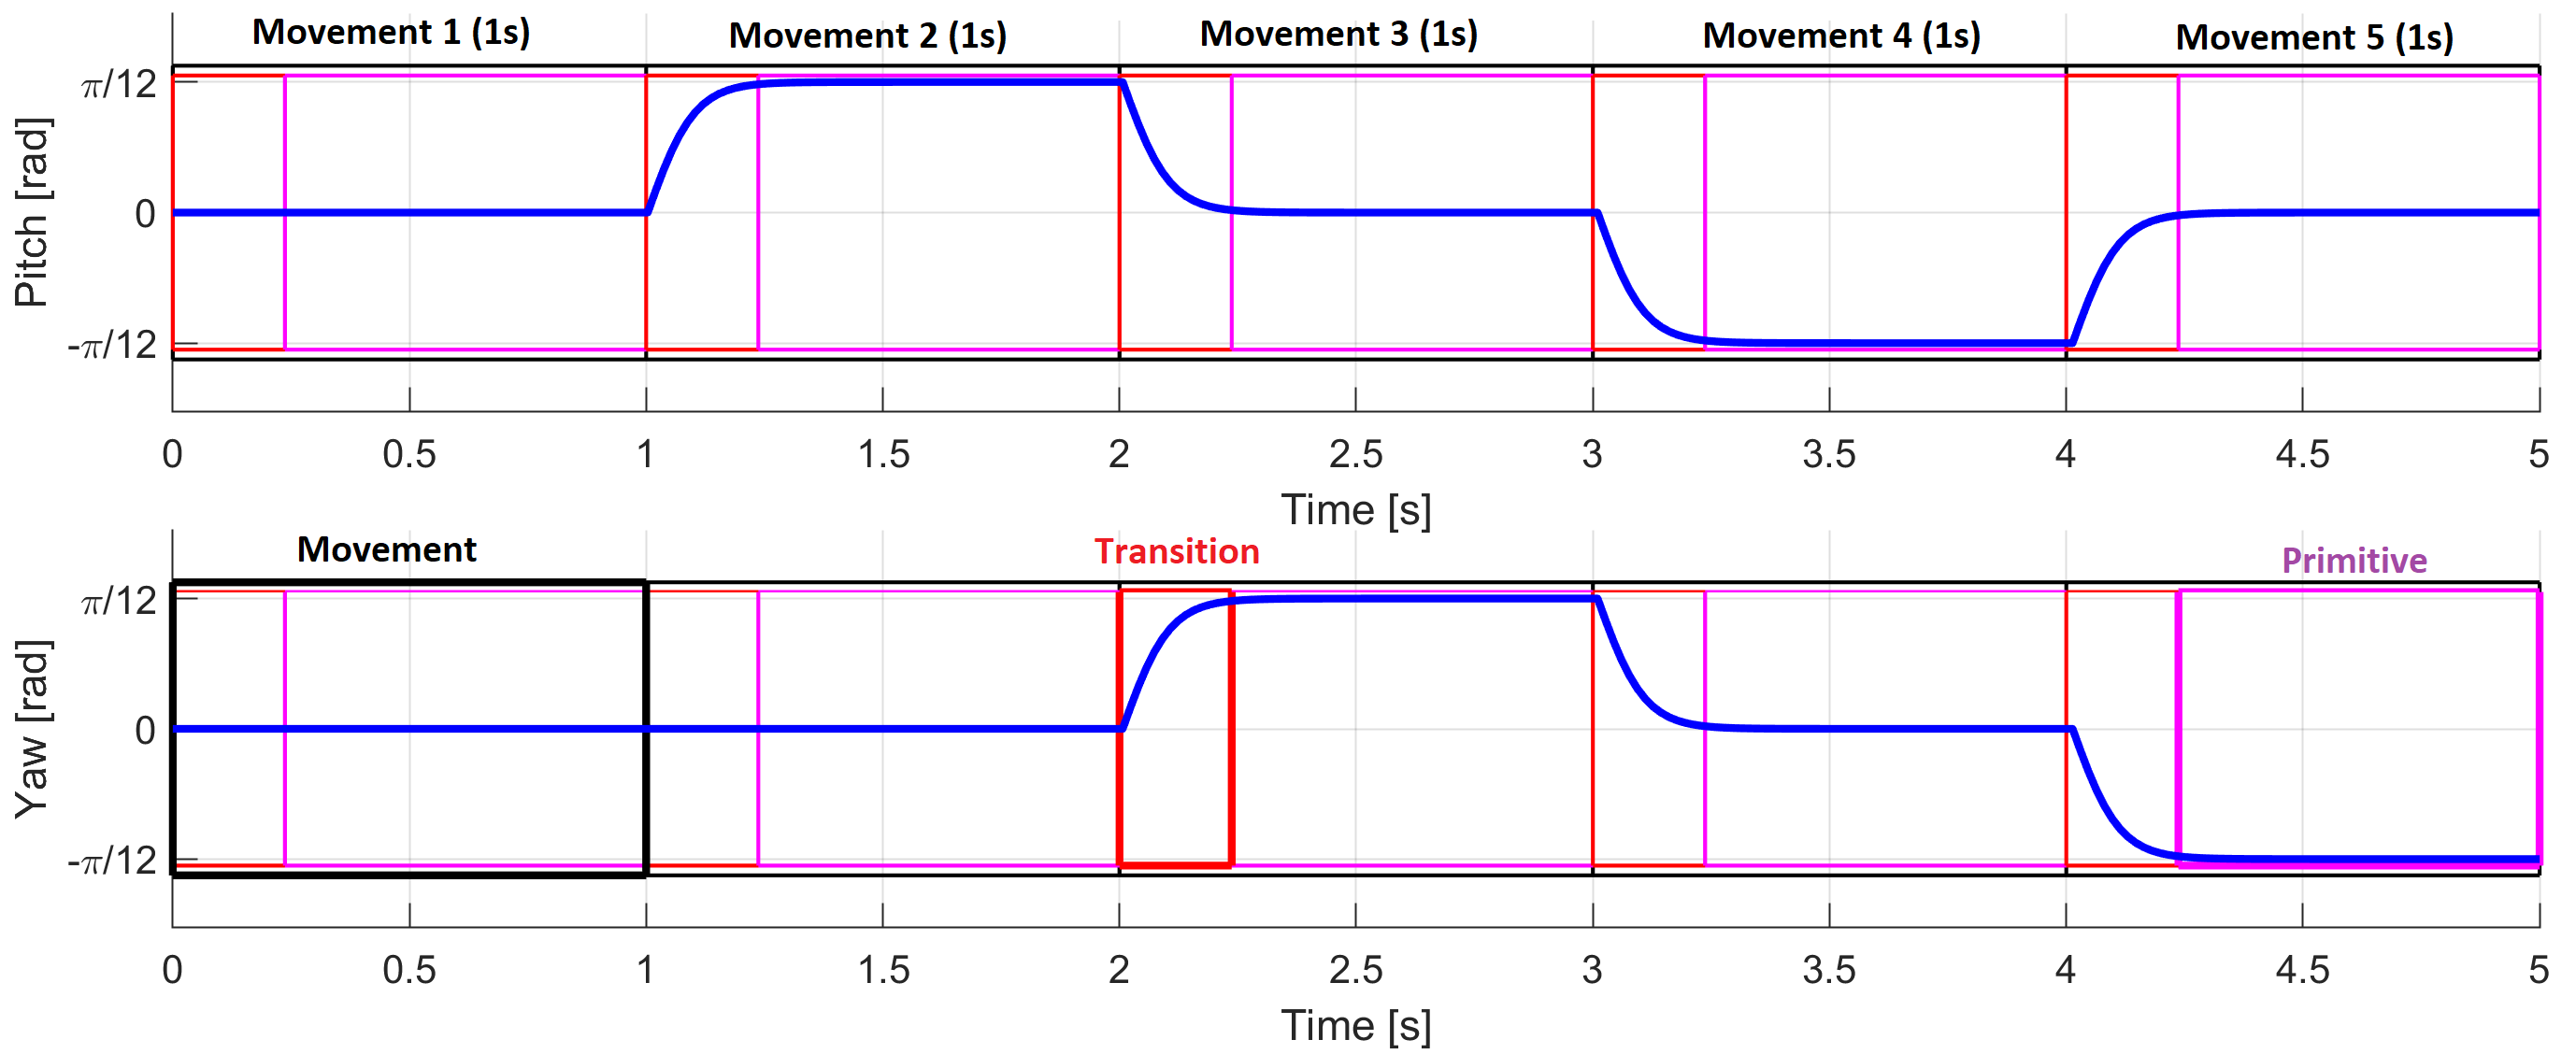
\includegraphics[width=0.95\linewidth]{\FIGDIR/TE062MovementAutomatonExampleWide} 
    \caption{Example of input signal segmentation to movements.}
    \label{fig:movementsExample}
\end{figure}

\begin{note}
    The hybrid automaton (sec. \ref{s:HybridAutomaton}) can be used as the base for simple control mechanism imitating navigators command execution by the pilot. The automaton states can be mapped to primitives and transitions. The reset map needs to be replaced with external order issuer to ensure smooth execution of commands.
    
    The future commands will be stacked in the buffer from which they will be picked for execution.
\end{note}



    \begin{definition}{Movement Primitive:}\label{def:MovementPrimitive}\\\emph{States} from \emph{Hybrid automaton} can be taken as \emph{Movements} in \emph{Movement Automaton}. \emph{MovementPrimitive} (eq. \ref{eq:movementPrimitive}) is describing the \emph{Movement} behavior as transfer function \emph{VectorField} enriched with parameters. 

    \begin{equation}\label{eq:movementPrimitive}
        \begin{aligned}
            &MovementPrimitive(vectorField,minimalDuration,parameters)\\
            &VectorField:SystemState\times parameters \to SystemState
        \end{aligned}
    \end{equation}
    \end{definition}



    \paragraph{Example: }Let say that \emph{UAS} system is given as $\dot{position}=velocity$, then let us have two \emph{MovementPrimitives}:
    
    \begin{enumerate}
        \item \textit{Stay} - $minimalTime=1s$, $parameters=\{\}$, $VectorField:\dot{position}=0$.
        \item \textit{Move} - $minimalTime=1s$, $parameters=\{velocity\}$, $VectorField:\dot{position}=velocity$.
    \end{enumerate}
    
    \paragraph{Trajectory from Movement Primitives:} The \emph{UAS} should \emph{Move} for $5s$ with velocity $10 m/s$, then \emph{Stay} for $10s$, then move for $7s$ with velocity $4 m/s$, with initial position $position_0=0$ and initial time $t_0=1$ The standard approach is to derive transfer function $position = \Theta(\dots)$
    \begin{equation}\label{eq:trajectoryExample}
        position(t)=\Theta(\dots)
        \begin{cases}
            t \in [0,5] &: 10\times t + position(0)\\
            t \in (5,15] &: 0\times (t-5) + position(5)\\
            t \in (15,22]&: 4\times (t-15) + position(15)
        \end{cases}
    \end{equation}

    The \emph{example} given by (eq. \ref{eq:trajectoryExample}) is fairly primitive, but imagine UAS system given by nonlinear dynamics \cite{fossen2011mathematical}. Then defining transfer function for a given command chain can be impossible.

    \begin{definition}{Movement Transition:}\label{def:movementTransition}\\
        \emph{System state} can be different from intended movement application, the notion of \emph{Transition} is therefore introduced as stabilizing element in movement chaining (eq. \ref{eq:movementTransition}).
        \begin{equation}\label{eq:movementTransition}
            Transition:MovementPrimitive\times SystemState \to MovementPrimitive    
        \end{equation}
    \end{definition}

    \paragraph{Trajectory with Transitions:} Introducing two transitions $Transition(Move,Stay)$ and $Transition(Stay,Move)$ reflecting periods when vehicle stop moving or speed-up to desired velocity. The transfer function (eq. \ref{eq:trajectoryExample}) can be rewritten as combination of \emph{MovementPrimitives} (eq. \ref{eq:movementPrimitive}) and \emph{Transitions} (eq. \ref{eq:movementTransition}):
    
    \begin{multline}
        Transition(Stay,Move), Move(5s,10m/s),\\
        Transition(Move,Stay), Stay(10s),\\ 
        Transition(Stay,Move), Move(7s,4m/s)
    \end{multline}.

    \begin{note} There are two types of \emph{movement primitives}:
    \begin{enumerate}
        \item \emph{Stationary} - when the system state is considered neutral, and they are considered an entry point for automaton.
        \item \emph{Dynamic} - when the system state is considered evolving, and they need to be terminated with a \emph{stationary} transition.
    \end{enumerate}
    \end{note}

    \paragraph{Movement Mapping Example:} Transition/MovementPrimitive pairs (eq. \ref{eq:movementTransition}) can be mapped into movements (eq. \ref{eq:movementMappingExample}).
    
    \begin{equation}\label{eq:movementMappingExample}
    \begin{aligned}
        Move(5s,10m/s) &:Transition(Stay,Move), Move(5s,10m/s),\\
        Stay(10s) &: Transition(Move,Stay), Stay(10s),\\ 
        Move(7s,4m/s) &: Transition(Stay,Move), Move(7s,4m/s)
    \end{aligned}    
    \end{equation}

    \begin{definition}{Movement:}\label{def:Movement}\\
        Movement can consist from multiple \emph{Transitions} (eq. \ref{eq:movementTransition}) and one \emph{MovementPrimitive} (eq. \ref{eq:movementPrimitive}), the duration of \emph{MovementPrimitive} can be shortened by \emph{Transitions} duration. \emph{Movement} is defined as follows:
        
        \begin{equation}
            \small Movement \left(
                \begin{gathered}
                    \scriptstyle initialState,\\
                    \scriptstyle initialTime[0..1],\\ 
                    \scriptstyle duration,\\ 
                    \scriptstyle parameters[0..1]
                \end{gathered}\right)
            = \small Chain \left(
            \begin{gathered}
            \small InitialTransition(\dots)[0..*],\\
            \small MovementPrimitive\left(
            \begin{gathered}
                \scriptstyle transitionState,\\
                \scriptstyle remainingDuration,\\
                \scriptstyle parameters
            \end{gathered}\right)\\
            \small LeaveTransition(\dots)[0..*],\\
            \end{gathered}
            \right)
        \end{equation}
        
        \emph{Chain function} connects multiple \emph{initial Transitions} which are applied at \emph{initialState} at \emph{initialTime}. Then own \emph{MovementPrimitive} (eq. \ref{eq:movementPrimitive}) is invoked with \emph{transitionnsState}. \emph{Transitions state} is state changed by \emph{Initial Transitions}. After \emph{Movement Primitive} there can be \emph{Leave Transitions Movement}
    \end{definition}

    \paragraph{Minimal Movement Time:} Given by (eq. \ref{eq:minimalMovementTime}) for \emph{movement} is given as the sum of \emph{MovementPrimitive} (eq. \ref{eq:movementPrimitive}) minimal time, and \emph{Transition} (eq. \ref{eq:movementTransition}) in/out combined minimal time.
    
    \begin{equation}\label{eq:minimalMovementTime}
        minimalTime(Movement)=
        \begin{aligned}
        &minimalTime(MovementPrimitive) +\\ &\text{max}_{in/out}\left\{time(Transition)\right\}
        \end{aligned}
    \end{equation}
   
    \paragraph{Movement Chaining:}\emph{Movements} can be \emph{chained} and applied to initial \emph{system state} to generate \emph{system trajectory}. Example of the trajectory is given by (eq. \ref{eq:trajectoryExample}). Movements are reversibly obtained by participation such a \emph{trajectory} into \emph{Movement primitives} and \emph{Transitions}. Then sample \emph{Trajectory} for $n\in \N^+$ movements looks like (eq. \ref{eq:movementChaining}).
    \begin{equation}\label{eq:movementChaining}
        \begin{aligned}
        &Trajectory(t_0)=State(t_0)\\
        &Trajectory(t_0,t_1]=Movement_1(Trajectory(t_0),t_0,duration_1,parameters_1)\\
        &Trajectory(t_1,t_2]=Movement_2(Trajectory(t_1),t_1,duration_2,parameters_2)\\
        &Trajectory(t_2,t_3]=Movement_3(Trajectory(t_2),t_2,duration_3,parameters_3)\\
        &\vdots\\
        &Trajectory(t_{n-1},t_n]=Movement_n(Trajectory(t_{n-1}),t_{n-1},duration_n,parameters_n)\\
        \end{aligned}
    \end{equation}

    Given \emph{Trajectory} at time $t_0$ is given as the initial \emph{State} of \emph{System}. For time interval $(t_0,t_1)$, which length is equal to $duration_1$, the \emph{State} is given by $Movement_1$ with $parameters_1$ and base time $t_0$. This behavior continues for movements $2,\dots,n$. 

    \begin{definition}{Movement Buffer:}\label{def:MovementBuffer}\\
        \noindent\emph{Movements} can be chained into \emph{Buffer} with the assumption of \emph{continuous movement execution}. \emph{Continuous movement executions} each movement in the chain (eq. \ref{eq:movementChaining}) is executed in time interval $\tau_i=(t_{i-1},t_{i}]$ where $i$ is movement order and $\forall$ $Movement_i$ starting time is $t_0$ or $t_{i-1}$ from the previous movement. With given assumption \emph{Buffer} is given as (eq. \ref{eq:movementBuffer}) with parameters $t_{i-1},t_{i}$ omitted, due $t_0$ and $duration_i$ dependency.
        
        \begin{equation}\label{eq:movementBuffer}
            Buffer = \left\{Movement_i(duration_i,parameters_i)\right\}i\in\N^+
        \end{equation}
    \end{definition}
    
    \begin{definition}{Movement Automaton Trajectory:}\label{def:MovementAutomatonTrajectory}\\
        Let say system \emph{State}$\in\R^n$ which \emph{Trajectory} is defined by movement chaining (eq. \ref{eq:movementChaining}), applied on some \emph{initial time} $t_0\in\R^+$ and final time $t_f=t_0+\sum_{i=1}^{I}duration_i$, with movements contained in \emph{Buffer} (eq. \ref{eq:movementBuffer}) is given as \emph{Trajectory} (eq. \ref{eq:TrajectoryDefinition}).
        
        \begin{equation}\label{eq:TrajectoryDefinition}
            Trajectory(t_0,State(t_0),Buffer)\text{ or } Trajectory(State_0,Buffer) \text{ if } t_0=0
        \end{equation}
    \end{definition}


    \begin{note}
        The space dimension of \emph{Trajectories} is $\R^{n+1}$ if the space dimension of state \emph{Space} is $R^n$, because \emph{Trajectory space} contains evolution of \emph{Space} in time interval $T[t_0,t_f]$.
        
        \noindent The transformation from \emph{transfer function} (eq. \ref{eq:trajectoryExample}) to \emph{trajectory} (eq. \ref{eq:TrajectoryDefinition}) is natural, only set of \emph{Movement primitives} (eq. \ref{eq:movementPrimitive}) and set of \emph{Transitions} (eq. \ref{eq:movementTransition}) is required.
    \end{note}

    \paragraph{State Projection:} \emph{Trajectory} (eq. \ref{eq:TrajectoryDefinition}) is natural evolution of space over time, then there exists \emph{StateProjection} function (eq. \ref{eq:stateprojection}) which returns \emph{State} for specific \emph{Time}.
    
    \begin{equation}\label{eq:stateprojection}
        StateProjection:Trajectory\times Time \to State(Time)
    \end{equation}


    	\newpage
\section{Formal Movement Automaton Definition}\label{s:MovementAutomatonDefinitionAndProperties}

    \begin{definition}\label{def:movementAutomaton}Movement Automaton is given as follow:
    
    \begin{align}   
        \label{eq:madInitialState}
        InitialState&: \in \R^h, h\in \N^+\\
        \label{eq:madSystemdefinition}
        System&: \dot{State}=f(Time,State,Input)\text{ or } vectorField\\
        \label{eq:madMovementPrimitive}
        Primitives &= \left\{MovementPrimitive_i\left(
                                \begin{aligned}
                                &vectorField,\\
                                &minimalDuration,\\
                                &parameters
                                \end{aligned}\right)
                            \right\} i \in \N^+\\
        \label{eq:madTransitions}
        Transitions&= \left\{Transition_j\left(
                                \begin{aligned}
                                    &MovementPrimitive_l,\\
                                    &MovementPrimitive_k
                                \end{aligned}\right)_{k\neq l}\right\} j\in N^+\\
        \label{eq:madMovements}
        Movements&= \left\{Movement_m\left[
                                \begin{aligned}
                                    &Transition_o[0..*],\\
                                    &MovementPrimitive_p\\
                                    &Transition_r[0..*],\\
                                \end{aligned}\right]_{o \neq r}\right\}  m\in N^+\\
        \label{eq:madBuffer}
        Buffer&= \left\{Movement_s(duration_s,parameters_s)\right\} s\in \N^+\\
        \label{eq:madExecuted}
        Executed&= \left\{Movement_s(duration_s,parameters_t)\right\} t\in \N^+\\
        \label{eq:madBuilder}
        Builder&:Movement \times MovementPrimitive \to Movement\\
        \label{eq:madTrajectory}
        Trajectory&:InitialState\times Movement^u \to State \times Time, u\in N^+\\
        \label{eq:madStateProjection}
        StateProjection&:Trajectory\times Time \to State(Time)  
    \end{align}
    
    \noindent \emph{System} (eq. \ref{eq:madSystemdefinition}) is given in form of \emph{differential equations} $\dot{x} = f(t,x,u)$ or \emph{other transformable equivalent}, with \emph{initial state} (eq. \ref{eq:madInitialState}).
    
    \emph{Movements} (eq. \ref{eq:movementChaining}) are defined as sequence of necessary \emph{initial transitions} (eq. \ref{eq:madTransitions}), \emph{movement primitive} (eq. \ref{eq:madMovementPrimitive}), and, \emph{leave transitions} (\ref{eq:madTransitions}).
    
    The \emph{Buffer} contains a set of \emph{movement primitives} (eq. \ref{eq:madMovementPrimitive}) to be executed in order to achieve the desired goal. \emph{Builder} (eq. \ref{eq:madBuilder}) assures that first \emph{movement primitive} (eq. \ref{eq:movementPrimitive})from \emph{Buffer} (eq. \ref{eq:madBuffer}) is transformed into \emph{next movement} (eq. \ref{eq:madMovements}) based on \emph{current movement} (eq.\ref{eq:madMovements}).
    
    \noindent The system \emph{trajectory} (eq. \ref{eq:madTrajectory}) is defined in (eq. \ref{eq:TrajectoryDefinition}). \emph{State projection} (eqs. \ref{eq:stateprojection},\ref{eq:madStateProjection}) is giving \emph{State} variable for time $t\in[t_0,t_{max}]$ where $t_max$ is given by:
    \begin{equation}
    t_{max}=t_0+\sum_{i=1,u}Buffer.Movement(i).movementDuration    
    \end{equation}
    \end{definition}
    
    \begin{note}{From Continuous Reach set to Movement Automaton Control Reach Set:}\label{eq:fromContRStoMARS}

\emph{The reach set $R$} (\ref{eq:reachSetExample1}) for system $\text{d}/\text{d} \text{t state} =model(state,input)$ with initial state $state_0=state(t_i)$ in time interval $[t_i,t_{i+1}[$  is with existing control strategy $input(t)\in Control Strategy(t)$. The reach set $R(state_0, t_0,t_1)$ where $t_1 > t_0$.
\begin{equation}\label{eq:reachSetExample1}
    R(state_0, t_0,t_1) = \bigcup \left\{state(s):input(s)\in Control Strategy(s), s\in (t_0,t_1]\right\} 
\end{equation}


\noindent\emph{The reach set $\mathscr{R}$} (\ref{eq:reachSetExample2}) of the system under the control of the \emph{movement automation} consist from the set of trajectories $Trajectory(initialState,buffer)$, which are executed in constrained time period $[t_i,t_{i+1}[$.
\begin{multline}\label{eq:reachSetExample2}
     ReachSet(state_0,t_i,t_{i+1})=\\\left\{Trajectory(state_0,buffer):\text{duration}(buffer) \le (t_{i+1}-t_i)\right\}
\end{multline}
\end{note}

\begin{note}{Weak Invariance:}

When the UAS is under the control of the movement automaton  for the obstacle avoidance problem,  by design of the avoidance algorithm, the trajectories of the UAS will not intersect any threat. This means that the controlled system $\text{d}/\text{d} \text{t state} =model(state,input)$ is \emph{weakly invariant} to the complement of the threats, and with respect to the free space. A pair $(state, SafeSpace)$, where $\text{d}/\text{d} \text{t state} =model(state,input)$ and $SafeSpace$ is a closed set, is weakly invariant if there exist controls such that a trajectory starting inside $State_0\in SafeSpace$ remains inside $State (t)\in SafeSpace$ \cite{blanchini1999set}.
 \end{note}




		\subsection{\secState{R}UAS Model}\label{s:UASNonlinearModel}
\paragraph{Motivation:} Simplified rigid body kinematic model will be used. This model have decoupled roll, yaw and pitch angles. The focus is on \emph{reach set approximation methods}, therefore \emph{UAS model} is simplified.

\paragraph{State Vector} (eq. \ref{eq:simple3dStatevector}) defined as positional state in euclidean position in right-hand euclidean space, where \emph{x, y, z} can be abstracted as latitude, longitude, altitude.
\begin{equation}\label{eq:simple3dStatevector}
    state = \left [ x,y,z, roll, pitch, yaw \right]^T
\end{equation}


\paragraph{Input Vector} (eq. \ref{eq:simple3dInputVector}) is defined as linear velocity of UAS $v$ and angular speed of rigid body $\omega_{roll}, \omega_{pitch},\omega_{yaw}$.

\begin{equation}\label{eq:simple3dInputVector}
    input = \left [ v, \omega_{roll}, \omega_{pitch},\omega_{yaw}\right ]^T
\end{equation}


\noindent Velocity vector function (eq. \ref{eq:simple3dvelocityDistribution})  is is defined through standard rotation matrix  and linear velocity $v$, oriented velocity [$v_x$, $v_y$, $v_z$] given by (eq. \ref{eq:UASNonlinearModelSimple}).

\begin{equation}\label{eq:simple3dvelocityDistribution}
    \begin{bmatrix}
    v_x\\
    v_y\\
    v_z\
    \end{bmatrix}
    =
    \begin{bmatrix}
         v\cos(pitch)\cos(yaw)\\
         v\cos(pitch)\sin(yaw)\\
         -v\sin(pitch)\\
    \end{bmatrix}
\end{equation}

\paragraph{UAS Nonlinear Model} (eq. \ref{eq:UASNonlinearModelSimple}) is given by \emph{first order equations:}

\begin{equation}\label{eq:UASNonlinearModelSimple}
    \begin{aligned}
        \frac{\text{d} x}{\text{d} time} &= v\cos(pitch)\cos(yaw);\\
        \frac{\text{d} y}{\text{d} time} &= v\cos(pitch)\sin(yaw);\\
        \frac{\text{d} z}{\text{d} time} &= -v\sin(pitch);\\
    \end{aligned}\\\quad\quad
    \begin{aligned}
        \frac{\text{d} roll}{\text{d} time} &= \omega_{roll};\\
        \frac{\text{d} pitch}{\text{d} time} &= \omega_{pitch};\\
        \frac{\text{d} yaw}{\text{d} time} &= \omega_{yaw};\\
    \end{aligned}
\end{equation}

\paragraph{Discretization} for \emph{fixed step} $k$ we start with discretization of the input variables:

\noindent The \emph{linear velocity} in text step is given:
\begin{equation}\label{eq:applyMovement}
    v(k+1) = v(k) +\delta v(k)
\end{equation}

\noindent The \emph{roll, pitch, yaw} for next step are given 

\begin{equation}\label{eq:applyMovement1}
    \begin{aligned}
        roll(k+1)  &= roll(k) + \delta roll(k)\\
        pitch(k+1) & = pitch(k) + \delta pitch(k)\\
        yaw(k+1) & = yaw(k) + \delta yaw(k)\\
    \end{aligned}    
\end{equation}

\noindent The $\delta v(k)$ is \emph{velocity change}, $\delta roll(k)$, $\delta pitch(k)$, $\delta yaw(k)$, are \emph{orientation changes} for current discrete step $k$. If the duration of \emph{transition} is $0 s$ (as. \ref{ass:transitionTime}) then 3D trajectory evolution in discrete time is given as: 

\begin{equation}\label{eq:applyMovement2}
    \begin{aligned}
        x(k+1)&= x(k) + v(k+1) \cos(pitch(k+1)) \cos(yaw(k+1)) & = \delta x(k)\\
        y(k+1)&= y(k) + v(k+1) \cos(pitch(k+1)) \sin(yaw(k+1)) & = \delta y(k)\\
        z(k+1)&= z(k) - v(k+1) \sin(pitch(k+1))                & = \delta z(k)\\
        time(k+1)& = time(k)+1                                & = \delta time(k)
    \end{aligned}    
\end{equation}

\noindent The $\delta x(k)$, $\delta y(k)$, $\delta z(k)$ are positional differences depending on \emph{input vector} for given discrete time $k$:
\begin{equation}\label{eq:ourImput}
    input(k) = \left[
                    \begin{gathered}
                    \delta x(k), \delta y(k), \delta z(k), \delta v (k),\\
                    \delta roll (k), \delta pitch(k), \delta yaw(k),\delta time (k)
                    \end{gathered} 
                \right]^T
\end{equation}

\noindent The \emph{state vector} for discrete time is given:
\begin{equation}\label{eq:ourState}
    state(k) = \left[
                    \begin{gathered}
                     x(k),  y(k),  z(k),  v (k),\\
                     roll (k),  pitch(k),  yaw(k), time (k)
                    \end{gathered} 
                \right]^T
\end{equation}


		\subsection{\secState{R}UAS Movement Automaton}\label{s:movementAutomatonDefinition}

\paragraph{Motivation:} An \emph{UAS Nonlinear Model} (eq. \ref{eq:UASNonlinearModelSimple}) can be modeled by \emph{Movement Automaton} (def. \ref{def:movementAutomaton}). 

\paragraph{Movement Primitives} by (def. \ref{def:MovementPrimitive})  are given as (eq. \ref{eq:movementPrimitive}). To define primitives the \emph{minimal time} is $1 s$. The \emph{maximal duration} is also $1s$.

\begin{note}
	Each movement primitive will last for fixed duration $1s$.
\end{note} 

\begin{assumption}\label{ass:transitionTime}
    Let assume that \emph{transition time} of \emph{roll, pitch, yaw, linear velocity} is $0 s$.
\end{assumption}

Under the assumption (as. \ref{ass:transitionTime}) the \emph{movement transitions} (def. \ref{def:movementTransition}) have zero duration. Therefore movement primitives can be considered as movements.

\begin{note}
    The assumption (as. \ref{ass:transitionTime}) can be relaxed under condition that \emph{path tracking controller exists}.
\end{note}

\paragraph{Movements} satisfying (def. \ref{def:Movement}), for the nonlinear model (eq. \ref{eq:UASNonlinearModelSimple}) reduced to \emph{discrete model} (eq. \ref{eq:uasLinearDiscreteModel}), are given by \emph{apply movements} function (eq. \ref{eq:applyMovement}, \ref{eq:applyMovement1}, \ref{eq:applyMovement2}).

\begin{equation}\label{eq:uasLinearDiscreteModel}
    state(k+1) = applyMovement(state(k), input(k)) 
\end{equation}

\paragraph{Movement Set} for discrete model (eq. \ref{eq:uasLinearDiscreteModel}) is defined as set of unitary movements on main axes (tab. \ref{tab:movements1}) and diagonal axes (tab. \ref{tab:movements2}). 

The maneuvering capability of several commercial small fixed wing UAS were merged together. The turning rate on horizontal/vertical is defined as $15^\circ$.

The deltas are posed in \emph{UAS body-fixed coordinate frame} (ap. \ref{sec:complementsOfAlgebra}) for discrete time $k$. 

\begin{table}[H]
    \centering
    \begin{tabular}{r||r|r|r|r|r}
    	\multirow{2}{*}{Parameter} & \multicolumn{5}{c}{Movement} \\\cline{2-6} 
                &    Straight  & Down & Up & Left  & Right   \\\hline\hline
        $\delta     x(k)[m]$           &    1.00	  & 0.98  & 0.98  & 0.98 & 0.98  \\\hline
        $\delta     y(k)[m]$           &    0	      & 0	  & 0	  & 0.13 & -0.13 \\\hline
        $\delta     z(k)[m]$           &    0	      & -0.13 & 0.13  &	0	 & 0     \\\hline
        $\delta  roll(k) [^\circ]$	   &    0	      & 0	  & 0	  & 0    & 0     \\\hline
        $\delta pitch(k) [^\circ]$     &    0	      & $15^\circ$  & -$15^\circ$ & 0	 & 0     \\\hline
        $\delta   yaw(k) [^\circ]$     &    0	      & 0	  & 0	  & $15^\circ$ & -$15^\circ$ \\
    \end{tabular}
    \caption{Input values for main axes movements.}
    \label{tab:movements1}
\end{table}
\begin{table}[H]
    \centering
    \begin{tabular}{r||r|r|r|r}
    	\multirow{2}{*}{Parameter} & \multicolumn{4}{c}{Movement} \\\cline{2-5} 
                    & Down-Left & Down-Right & Up-Left  & Up-Right   \\\hline\hline
        $\delta     x(k)[m]$           & 0.76  & 0.76  & 0.76 & 0.76  \\\hline
        $\delta     y(k)[m]$           & -0.13	& 0.13	& 0.13 & -0.13 \\\hline
        $\delta     z(k)[m]$           & -0.13 & -0.13 & 0.13 & 0.13  \\\hline
        $\delta  roll(k) [^\circ]$	& 0	    & 0	    & 0    & 0     \\\hline
        $\delta pitch(k) [^\circ]$     & -$15^\circ$ & -$15^\circ$ & $15^\circ$ & $15^\circ$     \\\hline
        $\delta   yaw(k) [^\circ]$    & $15^\circ$	& -$15^\circ$	& $15^\circ$ & -$15^\circ$ \\
    \end{tabular}
    \caption{Input values for diagonal axes movements.}
    \label{tab:movements2}
\end{table}

\begin{note}
    \emph{Movement set} in shorten form is given as
    \begin{equation}\label{eq:OurMovementSet}
        Movement Set= \left\{
        \begin{gathered}
            Straight, Left,Right, Up, Down,\\
            Down Left, Down Right,  Up Left,   Up Right
        \end{gathered}
        \right\}
    \end{equation}
\end{note}

\paragraph{Trajectory} by (def. \ref{def:MovementAutomatonTrajectory}) for initial time $time = 0$ , initial state $state(0)$ and \emph{Movement Buffer} (from def. \ref{def:MovementBuffer}):
\begin{equation}\label{eq:ourBuffer}
    Buffer = \left\{
                movement(j):
                \begin{aligned}
                    &movement(j)\in Movement Set (eq. \ref{eq:OurMovementSet}),\\
                    & j \in 1\dots n, n \in N^+
                \end{aligned}
            \right\}
\end{equation}

\begin{assumption}
    The buffer is always non-empty, ordered, finite list of \emph{movements}.
\end{assumption}

\begin{note}
  The buffer have finite count $n$ of movements stored. The buffer is the planning instrument used by higher level navigation/avoidance algorithm to control UAS (Control/Command interface) (fig. \ref{fig:AvoidanceFrameworkConceptNew}).
\end{note}

%\noindent Trajectory (eq. \ref{eq:ourTrajectoryImplementation}) is then %given as the time-series of discrete states:
%\begin{equation}\label{eq:ourTrajectoryImplementation}
%    Trajectory(state(0),Buffer)= \left\{\begin{gathered}state(0)+\sum_{j=0}%^{i-1} input(movement(j)):\\i \in\left\{1\dots |Buffer|+1\right\}, \%\movement(\cdot) \in Buffer\end{gathered}\right\}
%\end{equation}

The discrete trajectory (eq. \ref{eq:ourTrajectoryImplementation}) is ordered set of states bounded to discrete time $0\dots n$, where $n$ is movement count of \emph{Buffer}. Trajectory set has $n+1$ members defined like the following:

\begin{equation}
    \begin{aligned}
    T&rajectory(state(0),Buffer)=\\
        &\left\{
        \begin{aligned}
            state(0) &= state(0),\\
            state(1) &= apply Movement\left(state(0), movement(1)\right),  \\
            state(2) &= apply Movement\left(state(1), movement(2)\right),  \\
             \vdots  &= \vdots\\
            state(n-1) &= apply Movement\left(state(n-2), movement(n-1)\right),  \\
            state(n)   &= apply Movement\left(state(n-1), movement(n)\right)  \\
        \end{aligned}
        \right\}
    \end{aligned}
\end{equation}

\noindent The $apply Movement$ (eq. \ref{eq:uasLinearDiscreteModel}) is concatenation function for discrete UAS model.
		\section{\secState{R}Segmented Movement Automaton}\label{s:segmentedMovementAutomaton}
\paragraph{Motivation:} Constructing \emph{Movement Automaton} for more complex system can be tedious. Used \emph{Movement Automaton} for \emph{UAS system} (\ref{eq:UASNonlinearModelSimple}) has decoupled control which is not true for most of the copters/planes \cite{fossen2011mathematical}.

\paragraph{Partitioning UAS State Space:} Proposed movement automaton is defined by its Movement set (tab. \ref{tab:movements1},\ref{tab:movements2}). Those can be scaled depending on maneuverability in the  \emph{Initial state} $state(0)$:
\begin{enumerate}
    \item \emph{Climb/Descent Rate} $\delta pitch_{max}(k)$ - the maximal climb or descent rate for Up/Down movements.
    \item \emph{Turn Rate} $\delta yaw_{max}(k)$ - the maximal turn rate for Left/Right movement.
    \item \emph{Acceleration} $\delta v_{max}(k)$ - the maximal acceleration in cruising speed range.
\end{enumerate}

\begin{definition}{State Space partition}\label{def:stateSpacePartition}
    \emph{Maneuverability} is depending on \emph{Initial State}. There can not be the infinite count of \emph{Movement Automatons}.
    
    The state space $State Space \in \R^n$ can be separated into two exclusive subsets:
    \begin{equation}
        StateSpace = [ImpactStates, NonImpactingStates]
    \end{equation}
    
    The \emph{Impacting states} are states which bounds the \emph{Maneuverability}: $\delta pitch_{max}(k)$, $\delta yaw_{max}(k)$, $\delta v_{max}(k)$. For each \emph{impact state} is possible to define upper and lower boundary:
    \begin{multline}
        \forall impactState\in ImpactStates, \exists:\\ lower(impactState) \le value(impactState) \le upper(impactState) 
    \end{multline}
    
	\noindent    The bounded interval of impact state can be separated into distinctive \emph{impact state segments} like follow:
    \begin{multline}
        impactState\in [lower,upper]:\\ \{[lower,separator_1[\dots\cup\dots[separator_i,separator_{i+1}[\dots\cup\dots\\\dots\cup\dots[separator_n,upper]\}=\\
        = impactStateIntervals(impactState)
    \end{multline}
    \begin{note}
        The interval length depends on model dynamics. The rule of thumb is to keep maximal climb/descend/turn/acceleration rates near constant value. 
    \end{note}
      
\noindent When partitioning of \emph{all impact States} finishes, the count of partitions is given as product of \emph{count of partitions} for each member of \emph{Impact States}:
    
    \begin{equation}
        partition Count = \prod_{impactState \in}^{ImpactStates} |impactStateIntervals(impactState)| 
    \end{equation}
    
    \begin{note}
        Try to keep the count of partitions to minimum, each new interval increases the count of partitions geometrically. 
    \end{note}
    
    There is finite number $n$ of \emph{Impacting States}, these are separated into $impactState-$ $Intervals_i$ with respective index $i \in 1\dots n$. The \emph{segment} with index defining position used \emph{impacting state} intervals is given as \emph{constrained space}:
    
    \begin{equation}
        Segment(index) = \left[
            \begin{gathered}
                impactState_1 \in impactStateIntervals_1[index_1],\\
                \vdots\\
                impactState_n \in impactStateIntervals_n[index_n],\\
                \vdots\\
                NonImpactingStates    
                \end{gathered}\right]
    \end{equation}
    
    Each \emph{Segment} covers one of impacting state intervals combination, because the original intervals are exclusive, also \emph{Segments} are exclusive. The \emph{union} of all segments covers \emph{State Space}:
    
    \begin{equation}\label{eq:segmentedStateSpace}
        StateSpace = \bigcup_{\forall\quad index \in |impactStateIntervals|^n} Segment(index)
    \end{equation}
\end{definition}

\paragraph{Segmented Movement Automaton:} The segmentation of \emph{state space} is done  in (def. \ref{def:stateSpacePartition}) any \emph{state} belongs exactly to \emph{Segment} of \emph{State Space}. For each \emph{Segment} in \emph{State Space}it is possible to assess: \emph{Climb/Descent Rate} $\delta pitch_{max}(k)$, \emph{Turn Rate} $\delta yaw_{max}(k)$, and, \emph{Acceleration} $\delta v_{max}(k)$.


\begin{definition}{Movement Automaton for Segment(index)}\label{def:segmentMovementAutomaton}
    

\noindent For for Model(eq. \ref{eq:uasLinearDiscreteModel}) with State (eq. \ref{eq:ourState}) the input vector (eq. \ref{eq:ourImput}) is for position $[x,y,z]$ and velocity defined like: 

\begin{equation}
    \begin{aligned}
        \delta x(k)& = \left(v(k)+\delta v(k)\right) \cos(\delta pitch(k)) \cos(\delta yaw(k))\\
        \delta y(k)& = \left(v(k)+\delta v(k)\right) \cos(\delta pitch(k)) \sin(\delta yaw(k))\\
        \delta z(k)& = -\left(v(k)+\delta v(k)\right)\cos(\delta pitch(k))\\
        \delta v(k)&\in [-\delta v(k)_{max},\delta v(k)_{max}]
    \end{aligned}
\end{equation}
\end{definition}

\noindent The acceleration $\delta v(k)$ is in interval $[-\delta v(k)_{max},\delta v(k)_{max}]$, usually set to 0 $ms^{-1}$. The change of the orientation angles for \emph{Movement Set} (eq. \ref{eq:OurMovementSet}) is given in (tab. \ref{tab:movements3},\ref{tab:movements4}).

\begin{table}[H]
    \centering
    \begin{tabular}{r||r|r|r|r|r}
    
        $input(movement)$           &    Straight  & Down & Up & Left  & Right   \\\hline\hline
        $\delta  roll(k) [^\circ]$	   &    0	      & 0	  & 0	  & 0    & 0     \\\hline
        $\delta pitch(k) [^\circ]$     &    0	      & $\delta pitch_{max}$  & -$\delta pitch_{max}$ & 0	 & 0     \\\hline
        $\delta   yaw(k) [^\circ]$     &    0	      & 0	  & 0	  & $\delta yaw_{max}$ & -$\delta yaw_{max}$ \\
    \end{tabular}
    \caption{Orientation input values for main axes movements.}
    \label{tab:movements3}
\end{table}


\begin{table}[H]
    \centering
    \begin{tabular}{r||r|r|r|r}
        $input(movement)$             & Down-Left & Down-Right & Up-Left  & Up-Right   \\\hline\hline

        $\delta  roll(k) [^\circ]$	& 0	    & 0	    & 0    & 0     \\\hline
        $\delta pitch(k) [^\circ]$     & -$\delta pitch_{max}$ & -$\delta pitch_{max}$ & $\delta pitch_{max}$ & $\delta pitch_{max}$     \\\hline
        $\delta   yaw(k) [^\circ]$    & $\delta yaw_{max}$	& -$\delta yaw_{max}$	& $\delta yaw_{max}$ & -$\delta yaw_{max}$ \\
    \end{tabular}
    \caption{Orientation input values for diagonal axes movements.}
    \label{tab:movements4}
\end{table}

\begin{note}
    The \emph{Trajectory} is calculated same as in (eq. \ref{eq:ourTrajectoryImplementation}). The \emph{State Projection} is given as in (eq. \ref{eq:ourStateProjection}).
\end{note}

\noindent Then the \emph{Movement Automaton} for \emph{Segment} $\in$ \emph{State Space} is defined.

\begin{definition}{Segmented Movement Automaton}\label{def:segmentedMovementAutomaton}
    For system with segmented state space (eq. \ref{eq:segmentedStateSpace}) there is for each $state(k)$ in $StateSpace$ injection function:
    \begin{equation} \label{eq:activeMovementAutomaton}
        ActiveMovementAutomaton:StateSpace\to MovementAutomaton
    \end{equation}
    
\noindent Selecting appropriate \emph{movement automaton} implementation (def. \ref{def:segmentMovementAutomaton}) for \emph{state(k)} $\in$ \emph{Segment} $\subset$ \emph{State Space}. The mapping function (eq. \ref{eq:activeMovementAutomaton}) is injection mapping every state(k) to Segment then \emph{Movement Automaton Implementation}. The trajectory generated is then given:
    
    \begin{equation}\label{eq:ourTrajectoryImplementationSegmented}
        Trajectory\left(\begin{gathered}state(0),\\Buffer\end{gathered}\right)= 
        \left\{
            \begin{gathered}
                state(0)+\dots\\\sum_{j=0}^{i-1} 
                    \begin{aligned} 
                        &ActiveMovementAutomaton(state(j-1)).\\
                        &\quad.input(movement(j))
                    \end{aligned}:\\
                i \in\left\{1\dots |Buffer|+1\right\}, \\
                movement(\cdot) \in Buffer
            \end{gathered}
        \right\}
    \end{equation}
    
\end{definition}



		\section{\secState{R}Reference Trajectory Generator}\label{s:referenceTrajectoryGenerator}

\paragraph{Reference Trajectory Generator:} Segmented Movement Automaton (def.  \ref{def:segmentedMovementAutomaton}) with \emph{trajectory function} (eq. \ref{eq:ourTrajectoryImplementationSegmented}) is used as a \emph{reference trajectory generator} for \emph{complex systems}. 

There is an assumption that precise \emph{path tracking} implementation exist for such system which with \emph{thick reference trajectory} gives similar results to \emph{plain movement automaton control}.

The \emph{Reference trajectory} (eq. \ref{eq:generatedReferenceTrajectory}) for \emph{Planned} movement set is given as projection  of \emph{Trajectory} time series to position time series $[x,y,z,t]$:

\begin{equation}\label{eq:generatedReferenceTrajectory}
    Reference Trajectory:Trajectory\left(\begin{gathered}state(now),\\Planned\end{gathered}\right) 
    \to 
    \begin{bmatrix}
        x_{ref} \in \R^{|Planned|}\\
        y_{ref} \in \R^{|Planned|}\\
        z_{ref} \in \R^{|Planned|}\\
        t_{ref} \in \R^{|Planned|}
    \end{bmatrix}
\end{equation}

\paragraph{Predictor:} The \emph{Reference Trajectory Generator} (eq. \ref{eq:generatedReferenceTrajectory}) can also be used as a predictor. 

\begin{note}
    The \emph{Segmented Movement Automaton} (def. \ref{def:segmentedMovementAutomaton}) is used in this work with one Segment equal to State space with input function given by (\ref{tab:movements1}, \ref{tab:movements2}). The predictor used in \emph{Reach set computation} is given by (eq. \ref{eq:generatedReferenceTrajectory}).
\end{note}

\paragraph{State Projection} (eq. \ref{eq:ourStateProjection}) for the \emph{Trajectory} (eq. \ref{eq:ourTrajectoryImplementation}) is given as follow:
\begin{equation}\label{eq:ourStateProjection}
    StateProjection(Trajectory,time) = Trajectory.getMemberByIndex(time+1)
\end{equation}

\begin{note}
    \emph{Movement Automaton} for system (eq. \ref{eq:UASNonlinearModelSimple}) with given (as. \ref{ass:transitionTime}) is established with all related properties (sec. \ref{def:movementAutomaton}).
\end{note}
 
	
%% This adds a line for the Bibliography in the Table of Contents.
%\addcontentsline{toc}{chapter}{Bibliography}
%% *** Set the bibliography style. ***
%% (change according to your preference/requirements)
%\bibliographystyle{plain}
%% *** Set the bibliography file. ***
%% ("thesis.bib" by default; change as needed)
\bibliography{thesis}

%% *** NOTE ***
%% If you don't use bibliography files, comment out the previous line
%% and use \begin{thebibliography}...\end{thebibliography}.  (In that
%% case, you should probably put the bibliography in a separate file and
%% `\include' or `\input' it here).

\end{document}
